\section{Problema 1}
\subsection{Enunciado}
Debe de ingresar un vector de 10 elementos, llenarlo de números pares del 2 al 20. Al iniciar el
programa debe preguntar al usuario como quiere ver los números, el menú debe de ser por medio de
caracteres: “a”verlos de forma ascendente, “d”descendente, en caso que el usuario escriba otro valor
debe de decir que no es correcto y preguntarle el carácter nuevamente, hasta que este sea el correcto,
al ingresar el valor correcto muestra el vector en pantalla y termina el programa.

\subsection{Metodología}
Por un error de lectura del problema se realizó de modo que la única interacción con el usuario sea la parte de "ascendente" o "descendente". De este modo, se genera una lista con los números pares del $2$ al $20$ y se realiza un método \textit{shuffle} para randomizar la posición de los elementos de la lista, se utiliza como \textbf{seed} el "time(0)". Con esto, se utiliza la el método de ordenamiento merge sort. Ya dependiendo de la entrada del usuario se invierte el orden de la lista resultante o no.

\subsection{Variables de entrada y salida}
\begin{description}
	\item[$\rightarrow$: ] Caracter "A" o "D".
	\item[$\leftarrow$: ] lista de números. 
\end{description}

\subsection{Pseudocógido o Diagrama de Flujo}
\subsubsection{Algoritmo Merge Sort}
\paragraph{Función MergeSort(vector, incio, final)}
\begin{description}
	\item[Paso 1: ] Definimos donde queremos "partir" la lista: half = (inicio + final)$/2$
	\item[Paso 2: ] Se inicia la recursividad. Llamada a MergeSort(vector, inicio, half)
	\item[Paso 3: ] Llamada a MergeSort(vector, half $+$ 1, final)
	\item[Paso 4: ] Llamada a Merge(vector, inicio, half, final)
\end{description}

\paragraph{Función Merge(vector, inicio, half, final)}
\begin{description}
	\item[Paso 1: ] Se define una lista auxiliar y los iteradores i $=$ start, j $=$ half $+$ 1, k $=$ $0$ y t
	\item[Paso 2: ] Mientras $i \leq$ half $\& \&$ $j\leq$ final, hacer
	\begin{description}
		\item[Paso 2.1: ] k++. Si vector[i] $<$ vector[j] entonces auxiliar[k] = vector[i], i++.
		\item[Paso 2.2: ] En otro caso auxiliar[k] = vector[j], j++.
	\end{description}
	\item[Paso 3: ] Se agrega el elemento sobrante de alguna de las mitades al final de la lista auxiliar. (siempre habrá uno sobrante)
	\item[Paso 4: ] Reescribir todo en el vector original utlizando el contador "t".
\end{description}

\subsubsection{Algoritmo Shuffle}
\paragraph{Función shuffle(vector, length)}
\begin{description}
	\item[Paso 1: ] Se declaran variables locales "random\_ position", "step" y "k $=$ 0"
	\item[Paso 2: ] Mientras int $k <$ length hacer
		\begin{description}
			\item[Paso 2.1: ] random\_ position $=$ numero entero random $\in \, [0,\text{length} - 1]$
			\item[Paso 2.2: ] step $=$ vector[k]
			\item[Paso 2.3: ] vector[k] = vector[random\_ position]
			\item[Paso 2.4: ] vector[random\_ position] = step
		\end{description}
\end{description}

\subsubsection{Main}
\begin{description}
	\item[Paso 1: ] Generación del vector con elementos pares del 2 al 20
	\item[Paso 2: ] Aplicamos \textit{Shuffle} al vector para aleatorizarlo
	\item[Paso 3: ] Declaramos la variable de inicio del usuario y una variable control $=$ 0
	\item[Paso 4: ] Mientras control $==$ 0 hacer
	\begin{description}
			\item[Paso 4.1: ] Solicitar el ingreso del caracter "A" o "D"
			\item[Paso 4.2: ] Si es "A", aplicar MergeSort e imprimir el vector resultante. control = 1.
			\item[Paso 4.3: ] Si es "D", aplicar MergeSort e imprimir desde el final del vector hasta el inicio. control = 1.
			\item[Paso 4.4: ] Sino es ninguna, imprimir que no se ingresó ningún valor válido.
		\end{description}
\end{description}


\subsection{Código}
\begin{lstlisting}
//	Librerias
#include <stdio.h>
#include <stdlib.h>
#include <time.h>

// 0. Prototipado de funciones
void mergeSort(int main_array[], int start, int final);
void merge(int array[], int start, int half, int final);
void reverse(int array[], int length);
void printArrays(int array[], int length);
void shuffle(int array[], int length);
#define l 10

// 1. Funcion main

int main(){
  // 1.1. Definimos la "seed" como el tiempo, para el generador de numeros
  srand(time(0));

  // 2. Se crea un arreglo de numeros pares del 2 al 20
  int numeros[l];
  // 2.1. se ingresan los datos en la lista
  for (int i = 0; i < l; i++){ numeros[i] = 2*i + 2; }

  // 3. Se aleatoriza el arreglo
  printArrays(numeros, l);
  shuffle(numeros, l);
  printArrays(numeros, l);

  // 4. Interaccion con el usuario y ordenamiento del arreglo
  char input;
  int control = 0;
  while(control == 0){
    puts("Ingrese como desea ver los numeros.");
    puts("'A' para verlos de forma ascendente.");
    puts("'D' para verlos de forma descendente.");
    scanf("%s",&input);
    if (input == 65){
      control = 1;
      puts("WUUU FORMA ASCENDENTE");
      //printArrays(numeros, l);
      mergeSort(numeros, 0, l);
      printArrays(numeros, l);
    } else if (input == 68){
      control = 1;
      puts("WUUU FORMA DESCENDENTE");
      //printArrays(numeros, l);
      mergeSort(numeros, 0, l);
      reverse(numeros, l);
      printArrays(numeros, l);
    } else {
      puts("Ingrese un valor valido.");
    } // END IF
  } // END WHILE


  return 0;
} // END MAIN


/*
                              FUNCIONES UTILIZADAS
*/

void mergeSort(int main_array[], int start, int final){
  int half;
  half = (start + final)/2;
  if (start < final){
    mergeSort(main_array, start, half);
    mergeSort(main_array, half + 1, final);
    merge(main_array, start, half, final);
  } // END IF
} // END MERGESORT

void merge(int array[], int start, int half, int final){
  int aux[final + 1],i,j,k,t;

  k = 0; // movimiento por la lista auxiliar
  i = start; // movimiento por la sublista izquierda
  j = half + 1; // movimiento por la sublista derecha

  // ciclo para empezar a unir los arrays
  while(i <= half && j <= final){
    k++;
    if (array[i] < array[j]){
      aux[k] = array[i];
      i++;
    } else {
      aux[k] = array[j];
      j++;
    } // END IF
  } // END WHILE

  // para los elementos sobrantes de alguna de las sublistas
  for (t = i; t <= half; t++){
    k++;
    aux[k] = array[t];
  } // END FOR

  for (t = j; t <= final; t++){
    k++;
    aux[k] = array[t];
  } // END FOR

  // regresar todo al vector original
  for (t = 1; t <= k; t++){
    array[start + t - 1] = aux[t];
  } // END FOR
} // END MERGE

void reverse(int array[], int length){
  int aux[length];

  // Navegando el array del final hacia el inicio, y aux en forma contraria
  for (int i = length - 1; i >= 0; i--){
    aux[length - i - 1] = array[i];
  } // END FOR

  // regresando todo al vector original
  for (int j = 0; j < length; j++){
    array[j] = aux[j];
  } // END FOR
} // END INVERSE

void printArrays(int array[], int length){
  // impresion
  printf("(");
  for (int i = 0; i < length; i++){
    if (i != length - 1){
      printf("%d, ",array[i]);
    } else {
      printf("%d)\n", array[i]);
    } // END IF
  } // END FOR
} // END printArrays

void shuffle(int array[], int length){
  int random_position, step;
  for (int k = 0; k < length; k++){
    // Generamos una posicion random
    random_position = rand() % length;
    // intercambiar el actual elemento con el de la poiscion aleatoria
    step = array[k];
    array[k] = array[random_position];
    array[random_position] = step;
  } // END FOR
} // END SHUFFLE


// END PROGRAM
\end{lstlisting}



\section{Problema 2}
\subsection{Enunciado}
Crear un programa que solicite al usuario 5 números enteros, estos se deben de guardar en un vector,
al terminar de guardar los valores, el programa debe de ordenarlos de forma ascendente y mostrar el
vector ordenado. (utilice un método de ordenación.)

\subsection{Metodología}
Al igual que el problema anterior se utiliza el algoritmo merge sort, aunque se realizó una implementación de quick-sort y bubble-sort.

\subsection{Variables de entrada y salida}
\begin{description}
	\item[$\rightarrow$: ] 5 números \textbf{enterios} por parte del usuario.
	\item[$\leftarrow$: ] lista ordenada de números. 
\end{description}

\subsection{Pseudocógido o Diagrama de Flujo}
\begin{description}
	\item[Paso 1: ] Prototipado de funciones y definición de constantes, en este caso l = 5.
	\item[Paso 2: ] int vector[l]
	\item[Paso 3: ] Ingreso de los números por parte del usuario
	\item[Paso 4: ] Ordenar el vector con el algoritmo Merge Sort mostrado en el problema anterior.
	\item[Paso 5: ] Impresión del vector ordenado.
\end{description}

\subsection{Código}
\begin{lstlisting}
//	Librerias
#include <stdio.h>


// 0. Prototipado de funcion y definicion de variables
#define l 5
void mergeSort(int main_array[], int start, int final);
void merge(int array[], int start, int half, int final);
void printArrays(int array[], int length);

// 1. funcion main
int main(){
  // 3. declaracion de variables
  int vector[5];

  // 4. ingreso de datos
  puts("Ingrese 5 numeros enteros.");
  for (int i = 0; i < l; i++){ scanf("%d", &vector[i]); }

  // 5. Ordenamiento del array
  puts("Array ordenado.");
  mergeSort(vector, 0, l);
  printArrays(vector, l);

  return 0;
} // END MAIN


/*
                            FUNCITON
*/


void mergeSort(int main_array[], int start, int final){
  int half;
  half = (start + final)/2;
  if (start < final){
    mergeSort(main_array, start, half);
    mergeSort(main_array, half + 1, final);
    merge(main_array, start, half, final);
  } // END IF
} // END MERGESORT

void merge(int array[], int start, int half, int final){
  int aux[final + 1],i,j,k,t;

  k = 0; // movimiento por la lista auxiliar
  i = start; // movimiento por la sublista izquierda
  j = half + 1; // movimiento por la sublista derecha

  // ciclo para empezar a unir los arrays
  while(i <= half && j <= final){
    k++;
    if (array[i] < array[j]){
      aux[k] = array[i];
      i++;
    } else {
      aux[k] = array[j];
      j++;
    } // END IF
  } // END WHILE

  // para los elementos sobrantes de alguna de las sublistas
  for (t = i; t <= half; t++){
    k++;
    aux[k] = array[t];
  } // END FOR

  for (t = j; t <= final; t++){
    k++;
    aux[k] = array[t];
  } // END FOR

  // regresar todo al vector original
  for (t = 1; t <= k; t++){
    array[start + t - 1] = aux[t];
  } // END FOR
} // END MERGE

void printArrays(int array[], int length){
  // impresion
  printf("(");
  for (int i = 0; i < length; i++){
    if (i != length - 1){
      printf("%d, ",array[i]);
    } else {
      printf("%d)\n", array[i]);
    } // END IF
  } // END FOR
} // END printArrays


// END PROGRAM
\end{lstlisting}

\section{Problema 3}
\subsection{Enunciado}
Crear un programa que solicite al usuario dos posiciones en coordenadas (x,y,z) al obtenerlas debe de
almacenarlas en dos vectores, el programa automáticamente debe de mostrar los siguientes resultados:
\begin{multicols}{2}
	\begin{enumerate}[a)]
		\item magnitud de cada vector
		\item suma de los dos vectores
		\item producto escalar
		\item producto vectorial
	\end{enumerate}
\end{multicols}

\subsection{Metodología}
\begin{multicols}{2}
	\begin{enumerate}[a)]
		\item magnitud de cada vector: cálculo de magntidud de un vector
			$$\abs{\vec{v}} = \sqrt{v_x ^2 + v_y ^2 + v_z ^2}.$$
		\item suma de los dos vectores: para dos vectores $\vec{A} = (x_1,y_1,z_1)$ y $\vec{B} = (x_2,y_2,z_2)$.
			$$\vec{A} + \vec{B} = (x_1 + x_2,y_1 + y_2, z_1 + z_2).$$
		\item producto escalar: para los vectores anteriores
			$$\langle \vec{A} , \vec{B} \rangle = x_1 x_2 + y_1 y_2 + z_1 z_2.$$
		\item producto vectorial, dados los vectores anteriores
			$$\vec{A} \cp \vec{B} = \mqty{(y_1 z_2 - z_1 y_2) \vx \\ - (x_1 z_2 - z_1 x_2) \vy \\ + (x_1 y_2 - y_1 x_2) \vz} .$$
	\end{enumerate}
\end{multicols}

\subsection{Variables de entrada y salida}
\begin{description}
	\item[$\rightarrow$: ] Vectores $(x_1,y_1z_1)$ y $(x_2,y_2,z_2)$
	\item[$\leftarrow$: ] float para la magnitud, array para la suma, float para el producto escalar y array para el producto vectorial.
\end{description}

\subsection{Pseudocógido o Diagrama de Flujo}
\begin{figure}[H]
	\centering
	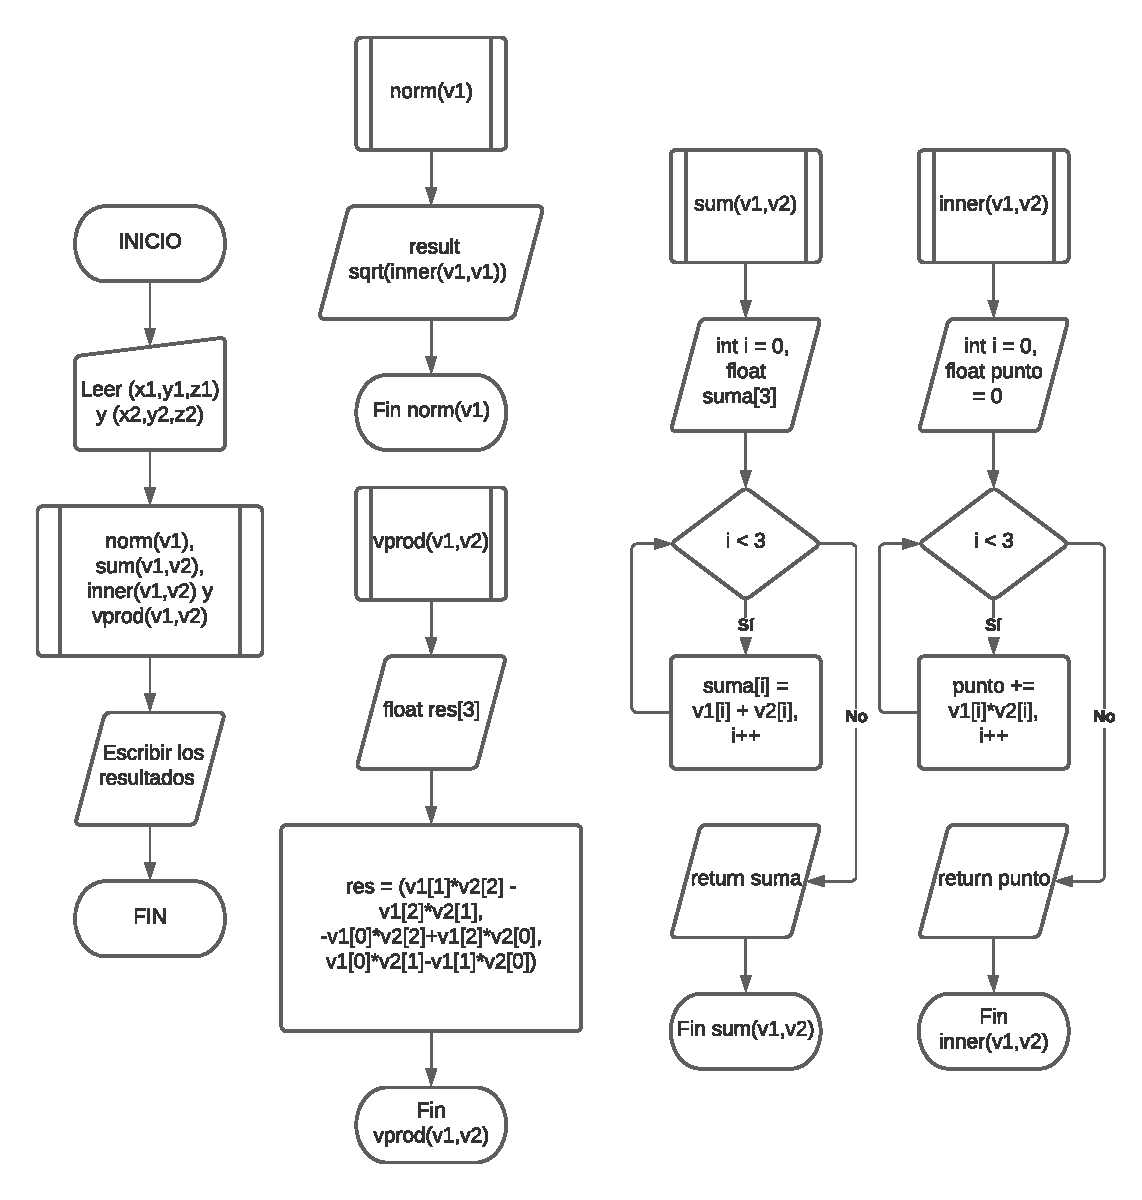
\includegraphics[scale=0.6]{img/problema3.pdf}
	\caption{Diagrama de flujo de las diferentes operaciones con vectores.}
	\label{DFp5}
\end{figure}


\subsection{Código}
\begin{lstlisting}
//	Librerias
#include <stdio.h>
#include <math.h>

// 0. Prototipado de funciones y declaracion de variables
//double sqrt(double x);
void printArrays(float array[], int length);
void suma_vectorial(float array1[], float array2[], float result[]);
float magnitud(float array[]);
float producto_interno(float array1[], float array2[]);
void producto_vectorial(float array1[], float array2[], float result[]);

// 1. Main function
int main(){
  // 2. declaracion de variables generales
  float vec1[3], vec2[3];
  float resvec[3];

  // 3. Ingreso de los vectores por parte del usuario
  puts("Ingrese dos vectores en R3 en la forma x1,x2,x3.");
  scanf("%f,%f,%f",&vec1[0],&vec1[1],&vec1[2]);
  scanf("%f,%f,%f",&vec2[0],&vec2[1],&vec2[2]);

  // 4. Realizando las diferente operaciones
  // 4.1. Suma de vectores
  suma_vectorial(vec1,vec2,resvec);
  puts("Suma de vectores.");
  printArrays(resvec, 3);
  // 4.2. magnitud de cada vector
  printf("Magnitud de cada vector. V1 = %f, V2 = %f\n", magnitud(vec1), magnitud(vec2));
  // 4.3. vector product
  producto_vectorial(vec1,vec2,resvec);
  puts("Producto vectorial entre ambos vectores.");
  printArrays(resvec, 3);
  // 4.4. inner product
  printf("Producto interno entre ambos vectores: %f\n",producto_interno(vec1,vec2));

  return 0;
} // END MAIN


/*
                          FUNCIONES
*/

float producto_interno(float array1[], float array2[]){
  float result = 0;

  for (int i = 0; i < 3; i++){
    result += array1[i]*array2[i];
  } // END FOR

  return result;
} // END PRODUCTO_INTERNO


void producto_vectorial(float array1[], float array2[], float result[]){
  // componentes del vector resultante
  result[0] = (array1[1]*array2[2] - array1[2]*array2[1]);
  result[1] = -(array1[0]*array2[2] - array1[2]*array2[0]);
  result[2] = (array1[0]*array2[1] - array1[1]*array2[0]);
} // END PRODUCTO_VECTORIAL


void printArrays(float array[], int length){
  // impresion
  printf("(");
  for (int i = 0; i < length; i++){
    if (i != length - 1){
      printf("%f, ",array[i]);
    } else {
      printf("%f)\n", array[i]);
    } // END IF
  } // END FOR
} // END printArrays


void suma_vectorial(float array1[], float array2[], float result[]){
  for (int i = 0; i < 3; i++){
    result[i] = array1[i]+array2[i];
  } // END FOR
} // END SUMA_VECTORIAL


float magnitud(float array[]){
  //double sqrt(double x);
  float norm = 0;

  for (int i = 0; i < 3; i++){
    norm += pow(array[i],2);
  } // END FOR
  return sqrt(norm);
} // END SUMA_VECTORIAL


// END PROGRAM
\end{lstlisting}


\section{Problema 4}
\subsection{Enunciado}
Crear un programa que solicite al usuario dos matrices de 3X3 almacenarlas como (matA, matB) y
una constante, el programa automáticamente debe de mostrar las los siguientes resultados:
\begin{multicols}{2}
	\begin{enumerate}[a)]
		\item Matriz A por constante
		\item Suma de las matrices
		\item Resta de las matrices
		\item Multiplicación de las matrices
		\item Determinante de la matriz A
		\item Transpuesta de la matriz B
		\item Inversa de la matriz A
		\item Reducción de Gauss de la matriz A
		\item Reducción de Gauss Jordan de la matriz B
	\end{enumerate}
\end{multicols}

\subsection{Metodología}
Sean $A = (a_{ij})$ y $B = (b_{ij})$, con ambas matrices $3\times 3$ y $c\in \R$.
\begin{multicols}{2}
	\begin{enumerate}[a)]
		\item Matriz A por constante. Cada elemento de la matriz multiplicado por la constante $c$.
			$$cA = (ca_{ij}).$$
		\item Suma de las matrices. Suma elemento a elemento, es decir
			$$A + B = (a_{ij} + b_{ij}).$$
		\item Resta de las matrices. Resta elemento a elemento, i.e.
			$$A - B = (a_{ij} - b_{ij}).$$
		\item Multiplicación de las matrices. Cada elemento de la matriz resultante $\Gamma = (\gamma _ {ij})$ es de la forma
			$$\gamma _{ij} = \sum _{k = 1} ^{n = 3} a_{ik} b_{kj}.$$
		\item Determinante de la matriz A. Tomando el método de cofactores, se define el menor como el determinante de una matriz $M_{ij}$ que resulta de quitar la $i-$ésima fila y la $j-$ésima columna de la matriz original. Dado esto, se define el cofactor asociacdo a $ij$, como $\mathcal{A}_{ij} = (-1)^{i+j} M_{ij}$. Y el determinante de la matriz se calcula multiplicando cada entrada de cualquier fila (o columna) por su respectivo cofactor, es decir (tomando la fila $1$ como ejemplo)
			$$\det{A} = \sum _{j = 1} ^3 (-1)^{1 + j} a_{1j} M_{1j}.$$
		Esta fue la implementación que se quizo hacer, dado que no se pudo por problemas en el código, se utilizó la regla de Sarrus
			$$ \det{A} = \qty(a_{11}a_{22}a_{33} + a_{12}a_{23}a_{31} + a_{13}a_{21}a_{32}) $$
			$$ - \qty(a_{31}a_{22}a_{13} + a_{32}a_{23}a_{11} + a_{33}a_{12}a_{21}). $$
			En dicha fórmula, los índices varían según la relación $i = (1+x) \mod{3}$ y $j = (2+x) \mod{3}$, con $x\in [0,2]$ (esto obviamente esta dedicado a la implementación, por eso los índices son 1 menos de lo que normalmente son.)
				$$\det{A} = \sum _{x = 0} ^2 a_{0x} \qty(a_{1i} a_{2j} - a_{1j} a_{2i}).$$
		\item Transpuesta de la matriz B. Se intercambian filas por columnas.
			$$B^t = (b_{ji}).$$
		\item Inversa de la matriz A. Para calcular la inversa se utiliza la siguiente relación
			$$A^{-1} = \frac{1}{\det{A}} \text{adj} (A).$$
		En donde la matriz $\text{adj} (A)$ es la matriz de cofactores transpuesta, en forma visual
			$$\text{adj} (A) = \text{cof} (A)^t = \mqty(\A _{11} & \A _{12} & \A _{13} \\ \A _{21} & \A _{22} & \A _{23} \\ \A _{31} & \A _{32} & \A _{33}) ^t.$$
		\item Reducción de Gauss de la matriz A. Es un método en el cual se busca reducir la matriz a una matriz escalonada, esta reducción se hace mediante operaciones entre filas y columnas, con el fin de llegar a una matriz triangular.
		$$ A_{\text{gauss}} = \mqty(a_{11} & a_{12} & a_{13} \\ 0 & a_{22} & a_{23} \\ 0 & 0 & a_{33}) $$
		\item Reducción de Gauss Jordan de la matriz B. Para este método es exactamente la misma idea que el anterior, con la savedad de que la matriz resultate es la identidad.
	\end{enumerate}
\end{multicols}

\subsection{Variables de entrada y salida}
\begin{description}
	\item[$\rightarrow$: ] Matrices $3\times 3$ $A$ y $B$, y constante $c \in \R$.
	\item[$\leftarrow$: ] Arrays bidimensionales y constantes, cada una en relación a cada inciso.
\end{description}

\subsection{Pseudocógido o Diagrama de Flujo}
\begin{figure}[H]
\centering
\subfigure["Main"]{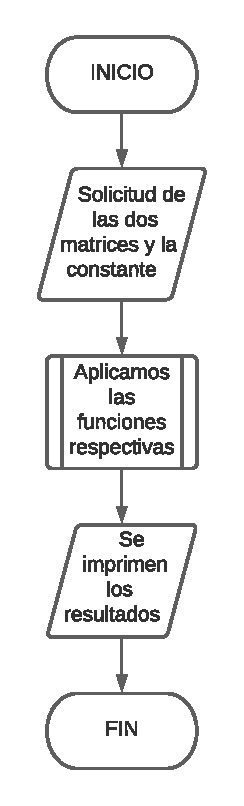
\includegraphics[scale=0.7]{img/problema4_1.pdf}}\qquad \qquad
\subfigure[Suma, resta y producto por escalar]{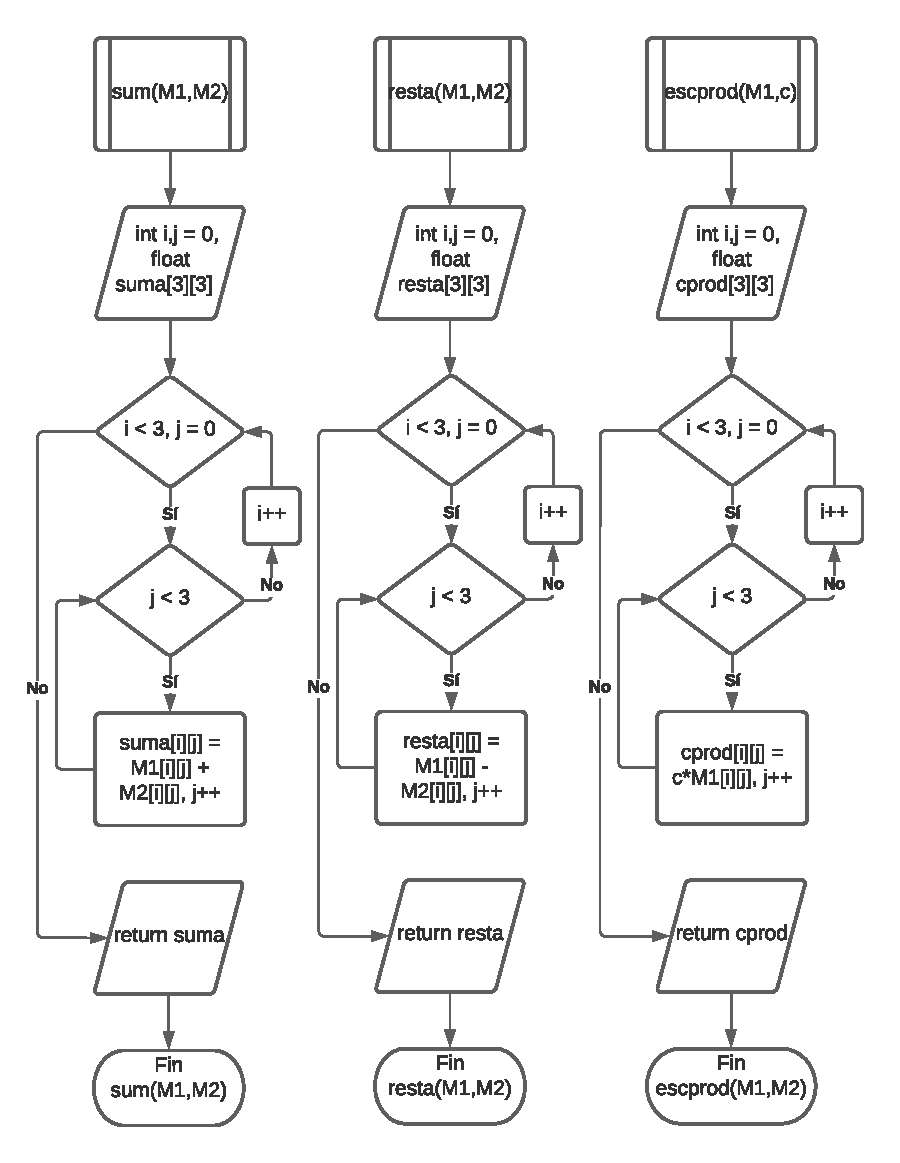
\includegraphics[scale=0.5]{img/problema4_2.pdf}}
\caption{(a) Diagrama de flujo de la función main. (b) Implementación de la suma y resta de matrices así como el producto por escalar.}
\label{FDp4}
\end{figure}

\begin{figure}[H]
\centering
\subfigure[Producto Matricial.]{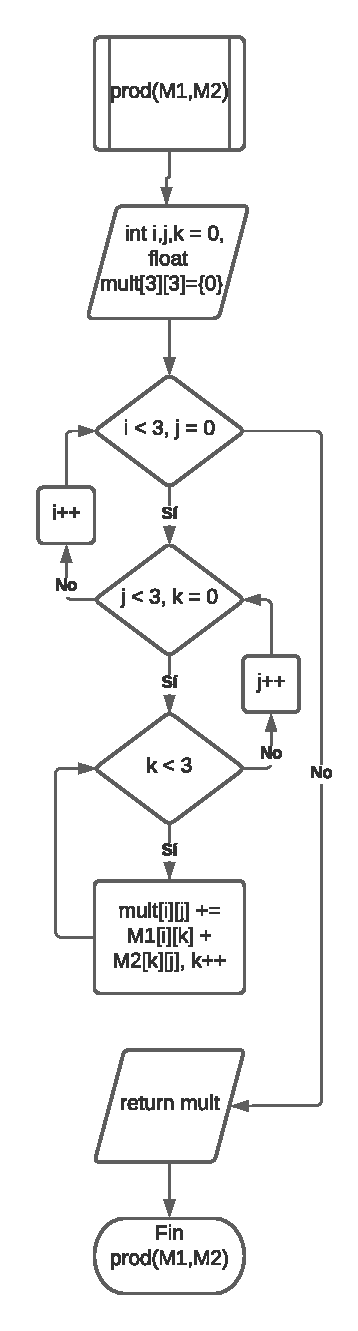
\includegraphics[scale=0.5]{img/problema4_3.pdf}}\qquad \qquad
\subfigure[Determinante, inversa y matriz de cofactores.]{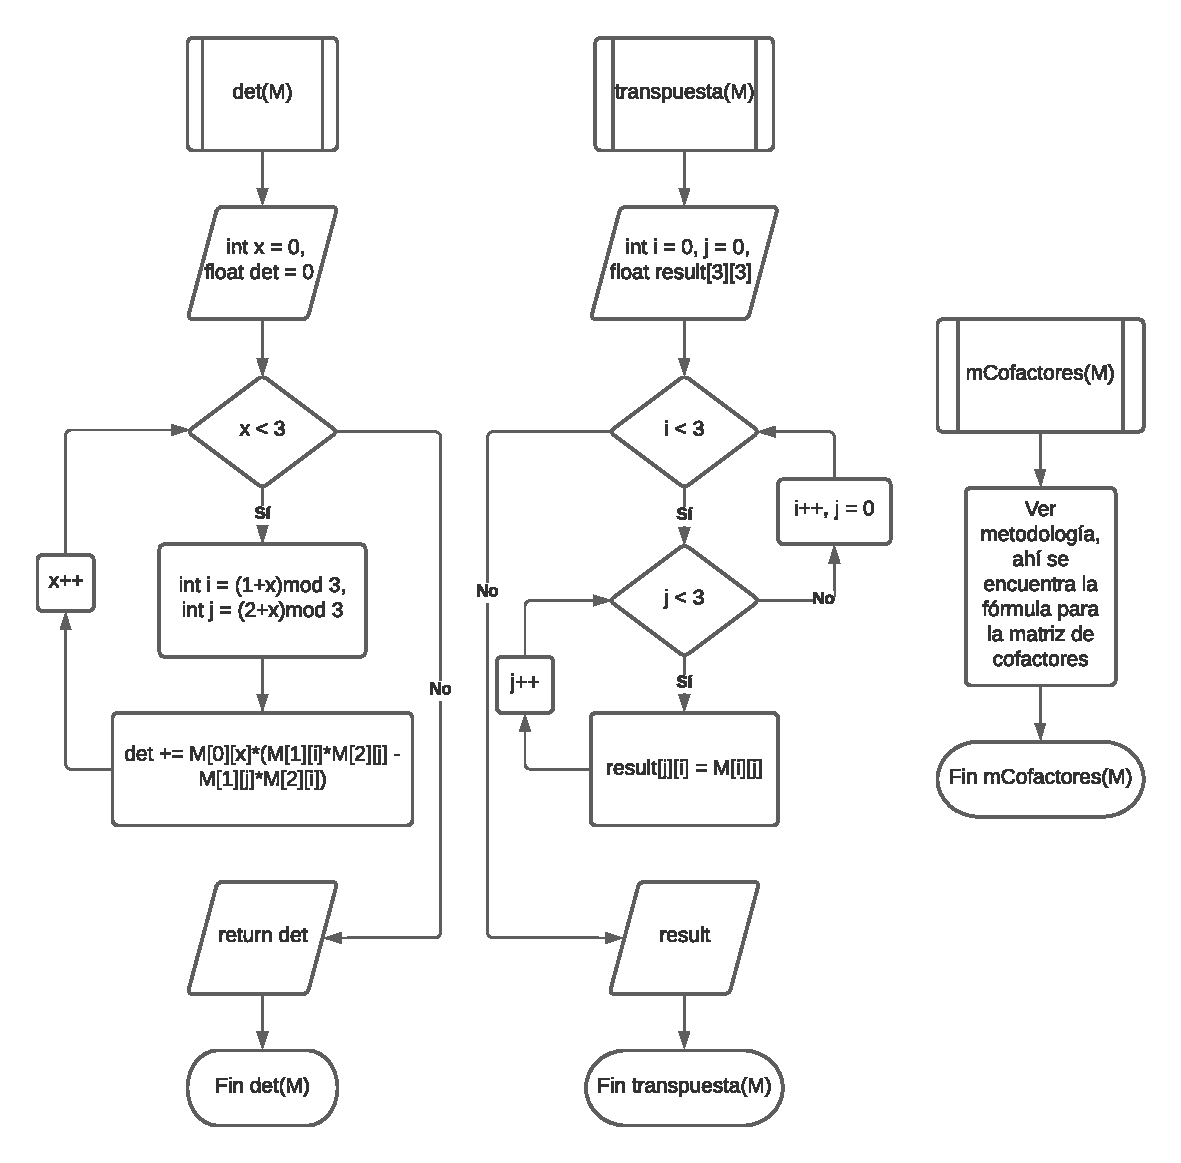
\includegraphics[scale=0.5]{img/problema4_4.pdf}}
\caption{(a) Producto de matrices según lo explicado en la metodología. (b) Determinante mediante la regla de Sarrus, cálculo de la matriz transpuesta y cálculo de la matriz de cofactores de manera directa (usando una fórmula).}
\label{FDp4}
\end{figure}

\subsection{Código}
\begin{lstlisting}
//	Librerias
#include <stdio.h>
#include <math.h>

// 0. prototipado de funciones (m filas y n columnas)
#define fila 3
#define col 3
void prod_escalar(float array[][col], int m, int n, float result[][col], float c);
void suma(float array1[][col], float array2[][col], int m, int n, float result[][col]);
void resta(float array1[][col], float array2[][col], int m, int n, float result[][col]);
void prod_matrices(float array1[][col], float array2[][col], int m, int n, float result[][col]);

float determinante(float array[][col]);
//float cofactor(float array[][col], int n, int file, int column);
void transpuesta(float array[][col], int m, int n, float result[][col]);
void mCofactores(float array[][col], float result[][col]);
void redGauss(float array[][col], float result[][col]);
void redGaussJordan(float array[][col], float result[][col]);

// 1. main
int main(){
  // 2. definiendo las variables a utilizar
  float matA[fila][col], matB[fila][col], result[fila][col], aux[fila][col];
  float c;

  // 3. ingreso de las matrices y la constante
  puts("Ingrese la primera matriz por filas en el siguiente formato: x,y,z");
  for (int i = 0; i < fila; i++){ scanf("%f,%f,%f", &matA[i][0], &matA[i][1], &matA[i][2]); }
  puts("Ingrese la primera matriz por filas en el siguiente formato: x,y,z");
  for (int j = 0; j < fila; j++){ scanf("%f,%f,%f", &matB[j][0], &matB[j][1], &matB[j][2]); }
  puts("Ingrese el valor de la constante.");
  scanf("%f",&c);
  puts("");
  // 4. calculo de los respectvos incisos
  // a)
  prod_escalar(matA, fila, col, result, c);
  puts("a) Matriz por una constante.");
  for (int i = 0; i < fila; i++){ printf("%f,%f,%f\n", result[i][0], result[i][1], result[i][2]); }
  puts("");

  // b)
  suma(matA, matB, fila, col, result);
  puts("b) matA + matB.");
  for (int i = 0; i < fila; i++){ printf("%f,%f,%f\n", result[i][0], result[i][1], result[i][2]); }
  puts("");

  // c)
  resta(matA, matB, fila, col, result);
  puts("c) matA - matB.");
  for (int i = 0; i < fila; i++){ printf("%f,%f,%f\n", result[i][0], result[i][1], result[i][2]); }
  puts("");

  // d)
  prod_matrices(matA, matB, fila, col, result);
  puts("d) matA * matB.");
  for (int i = 0; i < fila; i++){ printf("%f,%f,%f\n", result[i][0], result[i][1], result[i][2]); }
  puts("");

  // e)
  puts("e) det(matA).");
  printf("%f\n", determinante(matA));
  puts("");

  // f)
  transpuesta(matB, fila, col, result);
  puts("f) transpuesta de matB.");
  for (int i = 0; i < fila; i++){ printf("%f,%f,%f\n", result[i][0], result[i][1], result[i][2]); }
  puts("");

  // g)
  mCofactores(matA, result);
  transpuesta(result, fila, col, aux);
  prod_escalar(aux, fila, col, result, 1/determinante(matA));
  puts("g) inversa de matA.");
  for (int i = 0; i < fila; i++){ printf("%f,%f,%f\n", result[i][0], result[i][1], result[i][2]); }
  puts("");

  // h)
  redGauss(matA, result);
  puts("h) reduccion gauss de matA.");
  for (int i = 0; i < fila; i++){ printf("%f,%f,%f\n", result[i][0], result[i][1], result[i][2]); }
  puts("");

  // i)
  redGauss(matB, result);
  puts("i) reduccion gauss-jordan de matB.");
  for (int i = 0; i < fila; i++){ printf("%f,%f,%f\n", result[i][0], result[i][1], result[i][2]); }
  puts("");

  return 0;
} // END MAIN


/*
                            FUNCIONES
*/


void prod_escalar(float array[][col], int m, int n, float result[][col], float c){
  for (int i = 0; i < m; i++){
    for (int j = 0; j < n; j++){
      result[i][j] = c*array[i][j];
    } // END FOR
  } // END FOR
} // END prod_escalar


void suma(float array1[][col], float array2[][col], int m, int n, float result[][col]){
  for (int i = 0; i < m; i++){
    for (int j = 0; j < n; j++){
      result[i][j] = array1[i][j] + array2[i][j];
    } // END FOR
  } // END FOR
} // END suma


void resta(float array1[][col], float array2[][col], int m, int n, float result[][col]){
  for (int i = 0; i < m; i++){
    for (int j = 0; j < n; j++){
      result[i][j] = array1[i][j] - array2[i][j];
    } // END FOR
  } // END FOR
} // END suma


void prod_matrices(float array1[][col], float array2[][col], int m, int n, float result[][col]){
  for (int i = 0; i < m; i++){
    for (int j = 0; j < n; j++){
      result[i][j] = 0;
    } // END FOR
  } // END FOR

  for (int i = 0; i < m; i++){
    for (int j = 0; j < n; j++){
      for (int k = 0; k < n; k++){
        result[i][j] += array1[i][k] * array2[k][j];
      } // END FOR
    } // END FOR
  } // END FOR
} // END prod_matrices

// REGLA DE SARRUS
float determinante(float array[][col]){
  float det = 0;
  int i = 0, j = 0;

  for (int x = 0; x < 3; x++){
    i = (1 + x) % 3;
    j = (2 + x) % 3;

    det += array[0][x]*(array[1][i]*array[2][j] - array[1][j]*array[2][i]);
  } // END FOR
  return det;
} // END determinante


void transpuesta(float array[][col], int m, int n, float result[][col]){
  for (int i = 0; i < m; i++){
    for (int j = 0; j < n; j++){
      result[j][i] = array[i][j];
    } // END FOR
  } // END FOR
} // END transpuesta


void mCofactores(float array[][col], float result[][col]){
  // manualmente
  result[0][0] = array[1][1]*array[2][2] - array[1][2]*array[2][1];
  result[0][1] = -(array[1][0]*array[2][2] - array[1][2]*array[2][0]);
  result[0][2] = array[1][0]*array[2][1] - array[1][1]*array[2][0];
  result[1][0] = -(array[0][1]*array[2][2] - array[0][2]*array[2][1]);
  result[1][1] = array[0][0]*array[2][2] - array[0][2]*array[2][0];
  result[1][2] = -(array[0][0]*array[2][1] - array[0][1]*array[2][0]);
  result[2][0] = array[0][1]*array[1][2] - array[0][2]*array[1][1];
  result[2][1] = -(array[0][0]*array[1][2] - array[0][2]*array[1][0]);
  result[2][2] = array[0][0]*array[1][1] - array[0][1]*array[1][0];
} // END inversa


void redGauss(float array[][col], float result[][col]){
  result = array;
  for(int i=0;i<=2;i++){
        for(int j=3;j>=0;j--){
            result[i][j] = result[i][j]/result[i][i];
        } // END FOR
        for(int k=i+1;k<=2;k++){
            for(int j=3;j>=0;j--){
                result[k][j] = result[k][j] - result[k][i]*result[i][j];
            } // END FOR
        } // END FOR
    } // END FOR
} // END redGauss




void redGaussJordan(float array[][col], float result[][col]){
  result = array;
  for(int i=0;i<=2;i++){
        for(int j=3;j>=0;j--){
            result[i][j] = result[i][j]/result[i][i];
        }
        for(int k=i+1;k<=2;k++){
            for(int j=3;j>=0;j--){
                result[k][j] = result[k][j] - result[k][i]*result[i][j];
            }
        }
        for (int k=0; k<=i-1;k++){
            for(int j=3;j>=0;j--){
                result[k][j] = result[k][j] - result[k][i]*result[i][j];
            }
        }
    }
} // END redGaussJordan


// END PROGRAM
\end{lstlisting}



\section{Problema 5}
\subsection{Enunciado}
Crear un programa que encuentre el factorial de un numero entero ingresado, debe de utilizar una
función recursiva.

\subsection{Metodología}
La función factorial es una función recursiva definida a tramos
	$$n! = \left\{ \mqty{n*(n-1)! & n\geq 2 \\ 1 & n = 0,1 \\ 0 & \text{en otro caso.}} \right.$$
Existen muchas otras definiciones, como la función gamma, pero para interés del problema, utilizamos la definición recursiva.

\subsection{Variables de entrada y salida}
\begin{description}
	\item[$\rightarrow$: ] Número entero $n$.
	\item[$\leftarrow$: ] Número entero. (Dado el rápido crecimiento de la función factorial, es probable que para valores, aparentemente, normales de $n$, ni siquiera los \texttt{unsigned long long int} logren poder almacenar el número.)
\end{description}

\subsection{Pseudocógido o Diagrama de Flujo}
\begin{figure}[H]
	\centering
	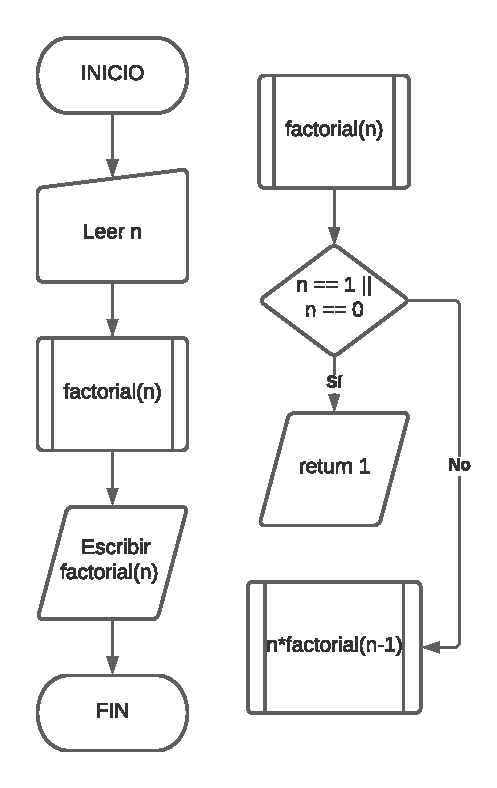
\includegraphics[scale=0.5]{img/problema5.pdf}
	\caption{Diagrama de flujo de la implementación recursiva de la función factorial.}
	\label{DFp5}
\end{figure}


\subsection{Código}
\begin{lstlisting}
//	Librerias
#include <stdio.h>

// 0. prototipado de funciones y definicion de variables
unsigned long long int factorial(int n);

// 1. funcion main
int main(){
  // 2. definicion de variables
  int n;

  // 3. ingreso y validacion del dato ingresado por el usuario
  puts("Ingrese un numero entero positivo.");
  scanf("%d", &n);

  //4. utilizacion de la funcion recursiva
  printf("El factorial del numero ingresado es: %lld\n", factorial(n));

  return 0;
} // END MAIN


/*
                          FUNCIONES
*/


unsigned long long int factorial(int n){
  if (n == 1 || n == 0){
    return 1;
  } else {
    return n*factorial(n-1);
  } // END IF
} // FUNCION FACTORIAL


// END PROGRAM
\end{lstlisting}


\section{Problema 6}
\subsection{Enunciado}
Crear un programa que realice la sumatoria desde 1 hasta un numero n que ingrese el usuario de las
siguientes funciones.
\begin{multicols}{2}
	\begin{enumerate}[a)]
		\item $$\sum _{k = 1} ^n k^2 (k - 3)$$
		\item $$\sum _{k = 2} ^n \frac{3}{k - 1}$$
		\item $$\sum _{k = 1} ^n \frac{1}{\sqrt{5}} \qty(\frac{1 + \sqrt{5}}{2})^k - \frac{1}{\sqrt{5}} \qty(\frac{1 - \sqrt{5}}{2})^k$$
		\item $$\sum _{k = 2} ^n 0.1(3\cdot 2^{k - 2} + 4).$$
	\end{enumerate}
\end{multicols}

\subsection{Metodología}
No hay mucho que añadir, la sumatoria es un bucle con almacenamiento en una variable que agrega el valor del paso anterior más el de la sucesión valuada en el $k$ correspondiente.

\subsection{Variables de entrada y salida}
\begin{description}
	\item[$\rightarrow$: ] Número entero $n$.
	\item[$\leftarrow$: ] Número entero o flotante, según sea el caso de la serie.
\end{description}

\subsection{Pseudocógido o Diagrama de Flujo}
\begin{description}
	\item[Paso 1: ] Prototipado de funciones para cada inciso (por simplicidad fueron nombradas con el inciso correspondiente), cuyas entradas son un número entero.
	\item[Paso 2: ] Ingreso del numero entero $n$ (limite superior de las series).
	\item[Paso 3: ] Para cada función se realizó exactamente el mismo procedimiento, solo que con diferente término de sumatoria, de modo que el ciclo for general es \\
	\texttt{Definir la suma como un float, $suma$} \\
	\texttt{Mientras un iterador sea menor igual que $n$, hacer}\\
	\texttt{suma $=$ suma $+$ $f_k$}\\
	\texttt{aumentar en $1$ el iterador}\\
	\texttt{Devolver "suma"}
	\item[Paso 4: ] Realizar esto para cada función e imprimir los respectivos resultados.
\end{description}


\subsection{Código}
\begin{lstlisting}
//	Librerias
#include <stdio.h>
#include <math.h>

// 0. Prototipado de funciones
float a(int n);
float b(int n);
float c(int n);
float d(int n);


// 1. funcion main
int main(){
  // 2. ingreso del limite superior
  int n;
  puts("Ingrese un numero entero positivo.");
  scanf("%d", &n);

  printf("Inciso a) %.2f \n", a(n));
  printf("Inciso b) %.2f \n", b(n));
  printf("Inciso c) %.2f \n", c(n));
  printf("Inciso d) %.2f \n", d(n));
}


/*
                            FUNCIONES
*/

float a(int n){
  float sum1 = 0;
  for (int i = 1; i <= n; i++){
    sum1 += pow(i,2)*(i - 3);
  }
  return sum1;
} //END a

float b(int n){
  float sum2 = 0;
  for (int i = 2; i <= n; i++){
    sum2 += 3/(i - 1);
  }
  return sum2;
} // END b

float c(int n){
  float sum3 = 0;
  for (int i = 1; i <= n; i++){
    sum3 += (1/sqrt(5))*pow(((1 + sqrt(5))/2),i) - (1/sqrt(5))*pow(((1 - sqrt(5))/2),i);
  }
  return sum3;
} // END c

float d(int n){
  float sum4 = 0;
  for (int i = 2; i <= n; i++){
    sum4 += 0.1*(3*pow(2,i - 2) + 4);
  }
  return sum4;
} // END d


// END PROGRAM
\end{lstlisting}













%%%%%%%%%%%%5